% nt-05-genealogy.tex

\documentclass[xcolor=dvipsnames]{beamer}
\usepackage{teachbeamer}

\title{Nietzsche and Genealogy}
\subtitle{{\CourseNumber}, {\CourseInst}}

\author{\CourseName}

\date{June 14, 2018}

\begin{document}

\begin{frame}
  \titlepage
\end{frame}

% \begin{frame}
%   \frametitle{iClicker Question}
% Choose from the following options. This item will be graded.
% \begin{block}{iClicker Question}
% [6595] Which geological epoch plays a special role in Bernard Williams' chapter about genealogy?
% \end{block}
% \begin{description}
% \item[A\hspace{.2in}$\blacktriangleright$] the pliocene
% \item[B\hspace{.2in}$\blacktriangleright$] the paleocene
% \item[C\hspace{.2in}$\blacktriangleright$] the pleistocene
% \item[D\hspace{.2in}$\blacktriangleright$] the holocene
% \end{description}
% \end{frame}

% \begin{frame}
%   \frametitle{iClicker Question}
% Choose from the following options. This item will be graded.
% \begin{block}{iClicker Question}
% [7252] What kind of story does Bernard Williams investigate in order to write a genealogy of truthfulness?
% \end{block}
% \begin{description}
% \item[A\hspace{.2in}$\blacktriangleright$] a children's story
% \item[B\hspace{.2in}$\blacktriangleright$] a literary story
% \item[C\hspace{.2in}$\blacktriangleright$] a state of nature story
% \item[D\hspace{.2in}$\blacktriangleright$] an autobiography
% \end{description}
% \end{frame}

% \begin{frame}
%   \frametitle{iClicker Question}
% Choose from the following options. This item will be graded.
% \begin{block}{iClicker Question}
% [1976] Which of these stories (genealogies) does Raymond Geuss tell in detail?
% \end{block}
% \begin{description}
% \item[A\hspace{.2in}$\blacktriangleright$] Modern Physics (via Planck and Einstein)
% \item[B\hspace{.2in}$\blacktriangleright$] Enlightenment (via Kant and Hume)
% \item[C\hspace{.2in}$\blacktriangleright$] Judaism (via Moses and Abraham)
% \item[D\hspace{.2in}$\blacktriangleright$] Christianity (via Paul and Jesus)
% \end{description}
% \end{frame}

% \begin{frame}
%   \frametitle{iClicker Question}
% Choose from the following options. This item will be graded.
% \begin{block}{iClicker Question}
% [3977] Raymond Geuss contrasts providing a genealogy with {\ldots}
% \end{block}
% \begin{description}
% \item[A\hspace{.2in}$\blacktriangleright$] {\ldots} giving a pedigree
% \item[B\hspace{.2in}$\blacktriangleright$] {\ldots} writing an autobiography
% \item[C\hspace{.2in}$\blacktriangleright$] {\ldots} compiling computer code
% \item[D\hspace{.2in}$\blacktriangleright$] {\ldots} composing a symphony
% \end{description}
% \end{frame}

\begin{frame}
  \frametitle{Truth and Truthfulness}
  Traditional theories of truth:
  \begin{enumerate}
  \item Correspondence Theory (what makes a belief true is its
    correspondence to a state in the world)
  \item Coherence Theory (what makes a belief true is the coherence of
    the belief system of which it is a part)
  \item Pragmatist Theory (truth is the end of inquiry; truth is
    satisfactory to believe)
  \end{enumerate}
  You may be a realist or an anti-realist (Michael Dummett) about
  truth. Deflationists about truth think that there is no metaphysical
  substance in the truth predicate because the proposition X and the
  proposition ``X is true'' are equivalent.
\end{frame}

\begin{frame}
  \frametitle{Geuss' View on Nietzsche and Truth}
  \begin{block}{Raymond Geuss: Nietzsche and Genealogy}
    If Nietzsche clearly attacks the correspondence view, shows no
    interest in coherence, and seems to present no clear alternative
    of his own invention, then he must tacitly hold some kind of
    reductivist or pragmatist view [according to Habermas]. The most
    fruitful way of taking Nietzsche seems to me to see him not as
    trying to propound his own variant theory of truth, but as
    formulating a new question ``How and why does the will-to-truth
    come about?'' (and claiming that this question is more interesting
    than, and doesn't presuppose an antecedent answer to Plato's
    question ``What is truth?''). (8)
  \end{block}
\end{frame}

\begin{frame}
  \frametitle{Truth and Truthfulness}
  It is difficult to keep the things that Nietzsche says about truth
  consistent. On the one hand, Williams lauds his attachment to the
  truth in so far as Nietzsche resists the cowardice of believing
  errors. On the other hand, Nietzsche is famously dismissive of
  objective and metaphysical truth.

  \bigskip

  Williams appears to be distinguishing between an attitude of
  \alert{truthfulness}, which is willing to believe something that is
  not useful or happymaking; and \alert{truth}, about whose origins
  there may be a genealogy.
  \begin{block}{Friedrich Nietzsche, The Gay Science, 167}
    We should not reinterpret the exceedingly derivative, late, rare,
    accidental, that we perceive only on the crust of the earth and
    make of it something essential, universal, and eternal. 
  \end{block}
\end{frame}

\begin{frame}
  \frametitle{Truth and Truthfulness}
  Key points about Nietzsche's attitude towards truth.
  \begin{itemize}
  \item ``fundamental insight: there is no pre-established harmony
    between the furthering of truth and the well-being of humanity''
    (does Nietzsche's view of truth square with his will to power
    monism?)
  \item ``it is still a metaphysical faith upon which our faith in
    science rests''
  \item ``error is not blindness---error is cowardice''
  \item nothing is really identical, all identity is a fiction (17)
  \item ``the antithesis of the apparent world and the true world is
    reduced to the antithesis world and nothing''
  \end{itemize}
\end{frame}

\begin{frame}
  \frametitle{Masking}
  \begin{block}{Michel Foucault: Histoire de la sexualit{\'e},
      page 113}
    C'est {\`a} la condition de masquer une part importante de
    lui-m{\^e}me que le pouvoir est tol{\'e}rable. Sa r{\'e}ussite
    est en proportion de ce qu'il parvient {\`a} cacher de ses
    m{\'e}canismes. Le pouvoir serait-it accept{\'e} s'il
    {\'e}tait enti{\`e}rement cynique? Le secret n'est pas pour
    lui de l'ordre de l'abus: il est indispensable {\`a} son
    fonctionnement.
  \end{block}
\end{frame}

\begin{frame}
  \frametitle{Genealogy I}
  \begin{block}{Bernard Williams: Truth and Truthfulness, 28}
  A genealogy is a narrative that tries to explain a cultural
  phenomenon by describing a way in which it came about {\ldots} Our
  ethical ideas are a complex deposit of many different traditions and
  social forces, and they have themselves been shaped by
  self-conscious representations of that history. However, the impact
  of these historical processes is to some extent concealed by the
  ways in which their product thinks of itself.
  \end{block}
\end{frame}

\begin{frame}
  \frametitle{Genealogy II}
  \begin{block}{Michel Foucault: Nietzsche, Genealogy, History, 142}
    However, if the genealogist refuses to extend his faith in
    metaphysics, if he listens to history, he finds that there is
    ``something altogether different'' behind things: not a timeless and
    essential secret, but the secrets that they have no essence or
    that their essence was fabricated in a piecemeal fashion from
    alien forms.
  \end{block}
\end{frame}

\begin{frame}
  \frametitle{Genealogy III}
    In the context of Hume's account of moral responsibility,
    genealogy denotes the kind of explanation pointing to the origins
    of a social practice of which it is essential that they themselves
    are not used as reasons to follow the practice. The core of the
    practice is somehow constituted by a certain forgetfulness toward
    its history. The forgetfulness is at the root of lending the
    practice intrinsic rather than instrumental value: a value which
    becomes detached from the original usefulness of the practice;
    also a value which experiences a threat to its reflective
    stability, and possibly a breakdown, when its historical origins
    are uncovered.
\end{frame}

\begin{frame}
  \frametitle{Genealogy IV}
Here are some examples for cultural phenomena (it may be very
controversial whether these really are cultural phenomena!) that have
been submitted to genealogies:
\begin{enumerate}
\item truth (Friedrich Nietzsche)
\item justice (David Hume)
\item morality (Friedrich Nietzsche)
\item gender (Judith Butler)
\item knowledge (Michel Foucault, Archaeology of Knowledge)
\item love (the prairie vole)
\item soul (Michel Foucault, The Body of the Condemned)
\end{enumerate}
\end{frame}

\begin{frame}
  \frametitle{Prairie Voles and Montane Voles}
  \begin{itemize}
  \item Prairie voles mate for life, and montane voles do not.
  \item Among prairie voles, the males not only share parenting
    duties, they will even lick and nurture pups that aren't their
    own.
  \item By contrast, male montane voles do not actively parent even
    their own offspring.
  \end{itemize}
  What accounts for the difference? Researchers have found that the
  prairie voles have greater numbers of oxytocin receptors in certain
  regions of the brain. Prairie voles that have had their oxytocin
  receptors blocked will not pair-bond. An object lesson in
  neuro-philosophy?
\end{frame}

\begin{frame}
  \frametitle{State of Nature Stories}
State of nature stories operate on simplified, imaginary environments.
  \begin{itemize}
  \item justice (D. Hume)
  \item state (R. Nozick)
  \item knowledge (E.J. Craig)
  \item truth (B. Williams)
  \item morality? (F. Nietzsche)
  \end{itemize}
  The state of nature is not the pleistocene. What characterizes
  humans naturalistically is their massive potential for non-genetic learning.
\end{frame}

\begin{frame}
  \frametitle{Just-So Stories}
  In 1902, Rudyard Kipling published a book called \emph{Just So
    Stories}. The term was appropriated in a derogatory fashion to
  discredit various types of evolutionary hypothesis about adaptation.
  The problem is usually that the hypothesis comes without means of
  empirical falsification.

  \bigskip

  \begin{tabular}{|c|c|c|}\hline
    & sons & daughters \\ \hline
    general-status mother & 2.8 & 1.7 \\ \hline
    low-status mother & 2.3 & 2.6 \\ \hline
  \end{tabular}

  \bigskip

  Trivers-Willard hypothesis. Williams makes the point that just-so
  stories may be fact-defective, but that doesn't automatically make
  them law-defective.
\end{frame}

\begin{frame}
  \frametitle{Function and Explanation}
  A property (such as altruism or other collaborative dispositions)
  may function to make individuals and the societies in which they
  live more fit. Williams correctly points out that functional
  accounts are not explanations. They lack historical plausibility
  since rational deliberation about the value of a property in the
  development of this property would beg the question. The prisoner
  dilemma illustrates this problem formally.

  \bigskip

  One way in which evolutionary psychology may overcome this problem
  is by introducing intrinsic (versus instrumental) goals. A parent
  does not come to the aid of a child because the well-being of the
  child is of instrumental value (in order to promote the gene
  propagation of near kin); the well-being of the child is of
  intrinsic value. This leads to a genealogy, which may either be
  vindicatory (Nozick: state) or non-vindicatory (Nietzsche:
  morality). 
\end{frame}

\begin{frame}
  \frametitle{Truth and Truthfulness}
  Williams' genealogy of truthfulness turns out to be vindicatory, and
  it entails that correspondence to facts is of intrinsic value.
  \begin{description}
  \item[truth] metaphysical, not historical
  \item[sincerity] historical, instrumental
  \item[truthfulness] historical, intrinsic
  \end{description}
\end{frame}

\begin{frame}
  \frametitle{Salvator Mundi: Pedigree or Genealogy}
      \begin{figure}[h]
    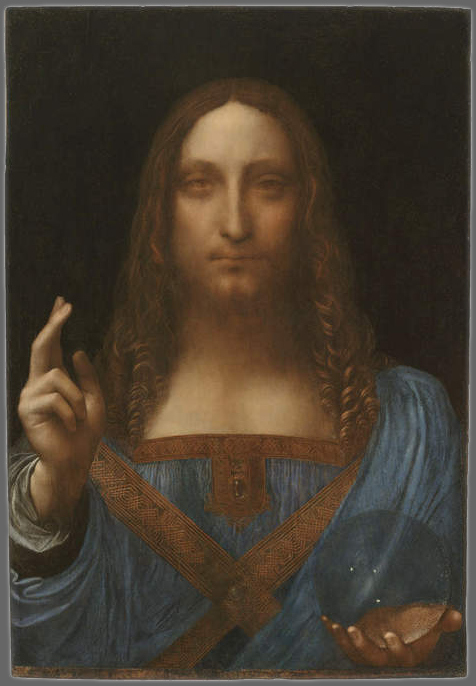
\includegraphics[scale=1]{./davinci_salvator-mundi_grt.jpg}
  \end{figure}
\end{frame}

\begin{frame}
  \frametitle{Salvator Mundi: Pedigree or Genealogy}
  \begin{enumerate}
  \item Louis XII of France (around 1500)
  \item Henrietta Maria (wife of Charles I of England, around 1625)
  \item John Stone (1651, for perhaps as little as 30 pounds)
  \item returned to Charles II of England (English Restoration, 1660)
  \item {\ldots} (third wives, illegitimate children, etc.) {\ldots}
  \item George III (1763)
  \item {\ldots} painting disappears {\ldots}
  \item Francis Cook (1900)
  \item sold for 45 pounds in 1958, painting disappears again
  \item Robert Simon purchases the painting for \$10,000 in 2005 at an
    auction in New Orleans
  \item Swiss dealer Yves Bouvier purchases the painting for
    \$75,000,000 in 2013
  \item Dmitry Rybolovlev immediately purchases the painting for
    \$127,500,000
  \item Mohammed bin Salman purchases the painting for \$450,312,500
    in 2017
  \end{enumerate}
\end{frame}

\begin{frame}
  \frametitle{Pedigree and Genealogy}
  These are characteristic features of a pedigree, to be contrasted
  with a genealogy according to Raymond Geuss.
  \begin{itemize}
  \item positive valorization
  \item linearity
  \item singular origin
  \end{itemize}
\end{frame}

\begin{frame}
  \frametitle{Genealogy of Christianity}
  As opposed to a pedigree of Christianity, in a genealogy of
  Christianity there 
  \begin{itemize}
  \item are diverse lines of development
  \item is a migration of concepts (the debtor-creditor relationship)
  \item is ``doused in blood'' (i.e.\ violent and oppressive)
  \item are contingencies (breaks, leaps, and coercions, GM II, 17)
  \item are individuals (Paul) and collectives (the Church, the
    mendicants) who impress their interpretation on a tradition
    (Foucault makes collective wills more precise with his theory of
    microdominations)
  \end{itemize}
\end{frame}

\begin{frame}
  \frametitle{iClicker Question}
Choose from the following options. This item will be graded.
\begin{block}{iClicker Question}
[1231] Which relationship develops on the basis of promisekeeping in Nietzsche's genealogy of morality?
\end{block}
\begin{description}
\item[A\hspace{.2in}$\blacktriangleright$] oligarch-plutocrat
\item[B\hspace{.2in}$\blacktriangleright$] infantry-cavalry
\item[C\hspace{.2in}$\blacktriangleright$] debtor-creditor
\item[D\hspace{.2in}$\blacktriangleright$] matrix-meretrix
\end{description}
\end{frame}

\begin{frame}
  \frametitle{iClicker Question}
Choose from the following options. This item will be graded.
\begin{block}{iClicker Question}
[6033] Fill in the blank: ``if a doctor had treated a {\ldots} for serious internal inflammations which would drive the European with the stoutest constitution to distraction; -- the do \emph{not} do that to the {\ldots}''
\end{block}
\begin{description}
\item[A\hspace{.2in}$\blacktriangleright$] Eskimo
\item[B\hspace{.2in}$\blacktriangleright$] Muscovite
\item[C\hspace{.2in}$\blacktriangleright$] Negro
\item[D\hspace{.2in}$\blacktriangleright$] Extraterrestrial
\end{description}
\end{frame}

\begin{frame}
  \frametitle{iClicker Question}
Choose from the following options. This item will be graded.
\begin{block}{iClicker Question}
[1507] Which words does Foucault use to illuminate the concept of genealogy?
\end{block}
\begin{description}
\item[A\hspace{.2in}$\blacktriangleright$] gen{\`e}se, origine, provenance
\item[B\hspace{.2in}$\blacktriangleright$] originem, formatio, cunabula
\item[C\hspace{.2in}$\blacktriangleright$] diathesis, syntaxis, katastasis
\item[D\hspace{.2in}$\blacktriangleright$] Ursprung, Entstehung, Herkunft
\end{description}
\end{frame}

\begin{frame}
  \frametitle{iClicker Question}
Choose from the following options. This item will be graded.
\begin{block}{iClicker Question}
[4256] In Foucault's paper ``Nietzsche, Genealogy, History,'' what kind of history is in contrast to traditional history?
\end{block}
\begin{description}
\item[A\hspace{.2in}$\blacktriangleright$] Gender history
\item[B\hspace{.2in}$\blacktriangleright$] effective history
\item[C\hspace{.2in}$\blacktriangleright$] poststructural history
\item[D\hspace{.2in}$\blacktriangleright$] Marxist history
\end{description}
\end{frame}

\end{document}
